\documentclass[11pt]{article}

\usepackage[margin=1in]{geometry}
\usepackage{amsfonts,amsmath}
\usepackage{booktabs}
\usepackage{graphicx}
\usepackage{xcolor}
\usepackage[colorlinks,citecolor=blue,urlcolor=blue,linkcolor=blue]{hyperref}
\usepackage[numbers,sort&compress]{natbib}

\renewcommand{\arraystretch}{1.3}
\emergencystretch=1.5em

\title{Supplementary Material for:\\
Construct Validity Failure in Single-Cell Embedding Evaluation:\\
Null Saturation Bounds and Source Classifier Confidence}

\author{Elliot Tower}
\date{}

\begin{document}
\maketitle

\setcounter{table}{0}
\renewcommand{\thetable}{S\arabic{table}}
\setcounter{figure}{0}
\renewcommand{\thefigure}{S\arabic{figure}}


\section{PBMC ceiling effect}
\label{app:pbmc}

The PBMC dataset \citep{ding2020systematic} provides seven scRNA-seq
technologies applied to the same donor PBMCs. Cell-type CKA ranges from
0.92 to 0.97 across all 28 source-target technology pairs. This
variance compression explains the null correlation with transfer F1
($\rho = +0.09$, $p = 0.87$): the metric cannot rank technologies on
a property where they score nearly identically. T cells, B cells, NK
cells, and monocytes are well-separated in any reasonable embedding; no
technology fails to capture this structure. The pancreas dataset contains
rare endocrine subtypes that are harder to resolve, providing sufficient
CKA variance for the correlation to emerge.


\section{Geometric modules}
\label{app:modules}

Five geometric modules for evaluating embedding transportability were
evaluated alongside the main metrics. Four were
eliminated by construct-validity checks: M1 (subspace overlap) and M6
(graph curvature) are confounded by embedding dimensionality via
Johnson--Lindenstrauss distance preservation; M2 (domain separability)
anti-predicts transfer; M4 (participation ratio) has
dimension-dependent normalization artifacts. M3 (direction stability)
was the sole candidate to survive construct-validity screening, but
achieves $\rho = +0.02$ ($p = 0.83$) on the full panel---no
predictive validity. These results demonstrate that the validity
protocol is non-trivial: it eliminates metrics, including those designed
by the protocol's authors.


\section{Spectral-gap experiment}
\label{app:spectral}

Null saturation could reflect either a normalization artifact fixable by
a better statistic, or a structural property of small-$k$ centroid
comparison. To distinguish these, we tested a spectral-gap ratio (SGR)
designed to exploit eigenvalue structure rather than Gram-matrix
alignment.

Random $k \times d$ matrices have flat singular-value spectra
(Marchenko--Pastur distribution). Cell-type centroid matrices from
trained models should have concentrated spectra---a few dominant
directions capturing biological axes such as immune versus
epithelial---producing higher explained-variance ratios than random.
For a $k \times d$ centroid matrix $C$, the spectral-gap ratio is
$\mathrm{SGR}_1 = s_1^2 / \sum_i s_i^2$ (fraction of variance in the
top singular value of the centered matrix). The discriminative
statistic is a $z$-score against $k,d$-matched null distributions
(5,000 Gaussian draws per pair).

Four hypotheses were tested: HS1
(discriminative): contender models have higher SGR $z$-scores than
baselines (Mann--Whitney $p < 0.05$). HS2 (predictive): SGR $z$-score
correlates with transfer F1 (partial $\rho > 0.20$, permutation
$p < 0.05$). HS3 (incremental): SGR adds variance beyond CKA. HS4
(both axes): HS1 and HS2 simultaneously.

The experiment produces a clean negative result across 22 tissues,
136 conditions, and 8 embedding models (Table~\ref{tab:sgr}). Null
baselines (random projection, untrained encoder) exhibit \emph{higher}
spectral concentration than trained models: baseline mean $z_1 = 141$,
contender mean $z_1 = 88$ (Mann--Whitney $U = 1{,}058$, one-sided
$p > 0.99$). SGR does not predict transfer (partial $\rho = -0.11$,
$p = 0.99$) and adds no information beyond CKA (partial
$\rho = 0.001$, $p = 0.99$). All four hypotheses fail.

\medskip
\medskip
\begin{table}[h!]
\centering
\caption{Spectral-gap test results (SGR$_1$ $z$-scores against
$k,d$-matched Gaussian null). Higher $z$ = more concentrated spectrum.
Trained models have \emph{lower} spectral concentration than
baselines.}
\label{tab:sgr}
\small
\begin{tabular}{@{}lcccl@{}}
\toprule
Model & $n$ & $z_1$ mean & SGR$_1$ mean & Role \\
\midrule
bog\_pca\_512           & 22 & 167 & 0.529 & contender \\
untrained encoder       & 22 & 155 & 0.498 & baseline \\
random projection       & 22 & 126 & 0.434 & baseline \\
scGPT                   & 22 & 76  & 0.311 & contender \\
Geneformer              & 22 & 65  & 0.275 & contender \\
scVI                    & 22 & 18  & 0.364 & contender \\
\bottomrule
\end{tabular}
\end{table}

The reversal has a clear mechanism. Random projections and untrained
encoders preserve the dominant variance axis of the input gene-expression
matrix (the immune--epithelial split that dominates transcriptomic
variation). Trained models redistribute variance across embedding
dimensions to separate cell types more evenly---precisely the
representation geometry that improves downstream classification but
lowers spectral concentration. Null saturation is structural: it
arises because \emph{any} projection of biologically structured
gene-expression data produces centroid matrices with concentrated
spectra, regardless of whether the model learned meaningful
representations.


\section{Noise dose-response}
\label{app:noise}

A metric suitable for certification should decrease monotonically as the
embedding is degraded. We tested this by adding Gaussian noise at seven
levels ($\sigma \in \{0.01, 0.05, 0.1, 0.25, 0.5, 1.0, 2.0\} \times$
embedding standard deviation) to six embedding methods across 22
tissues (120 conditions, 10 independent noise seeds per condition).

Each condition was evaluated using an $H$-statistic defined as
$H = \max_{\sigma > 0}[m(\sigma) - m(0)]$, the maximum increase in
the metric over baseline across noise levels. $H > 0$ indicates
non-monotonicity: the metric \emph{increased} at some noise level.
Raw positivity counts conditions where $H$ exceeds 0.01 averaged across
seeds. Calibrated positivity applies a permutation null (1{,}000
$\sigma$-label permutations per seed, $\alpha = 0.01$) to
distinguish genuine non-monotonicity from clustering jitter
(Table~\ref{tab:noise}).

\begin{figure}[h!]
\centering
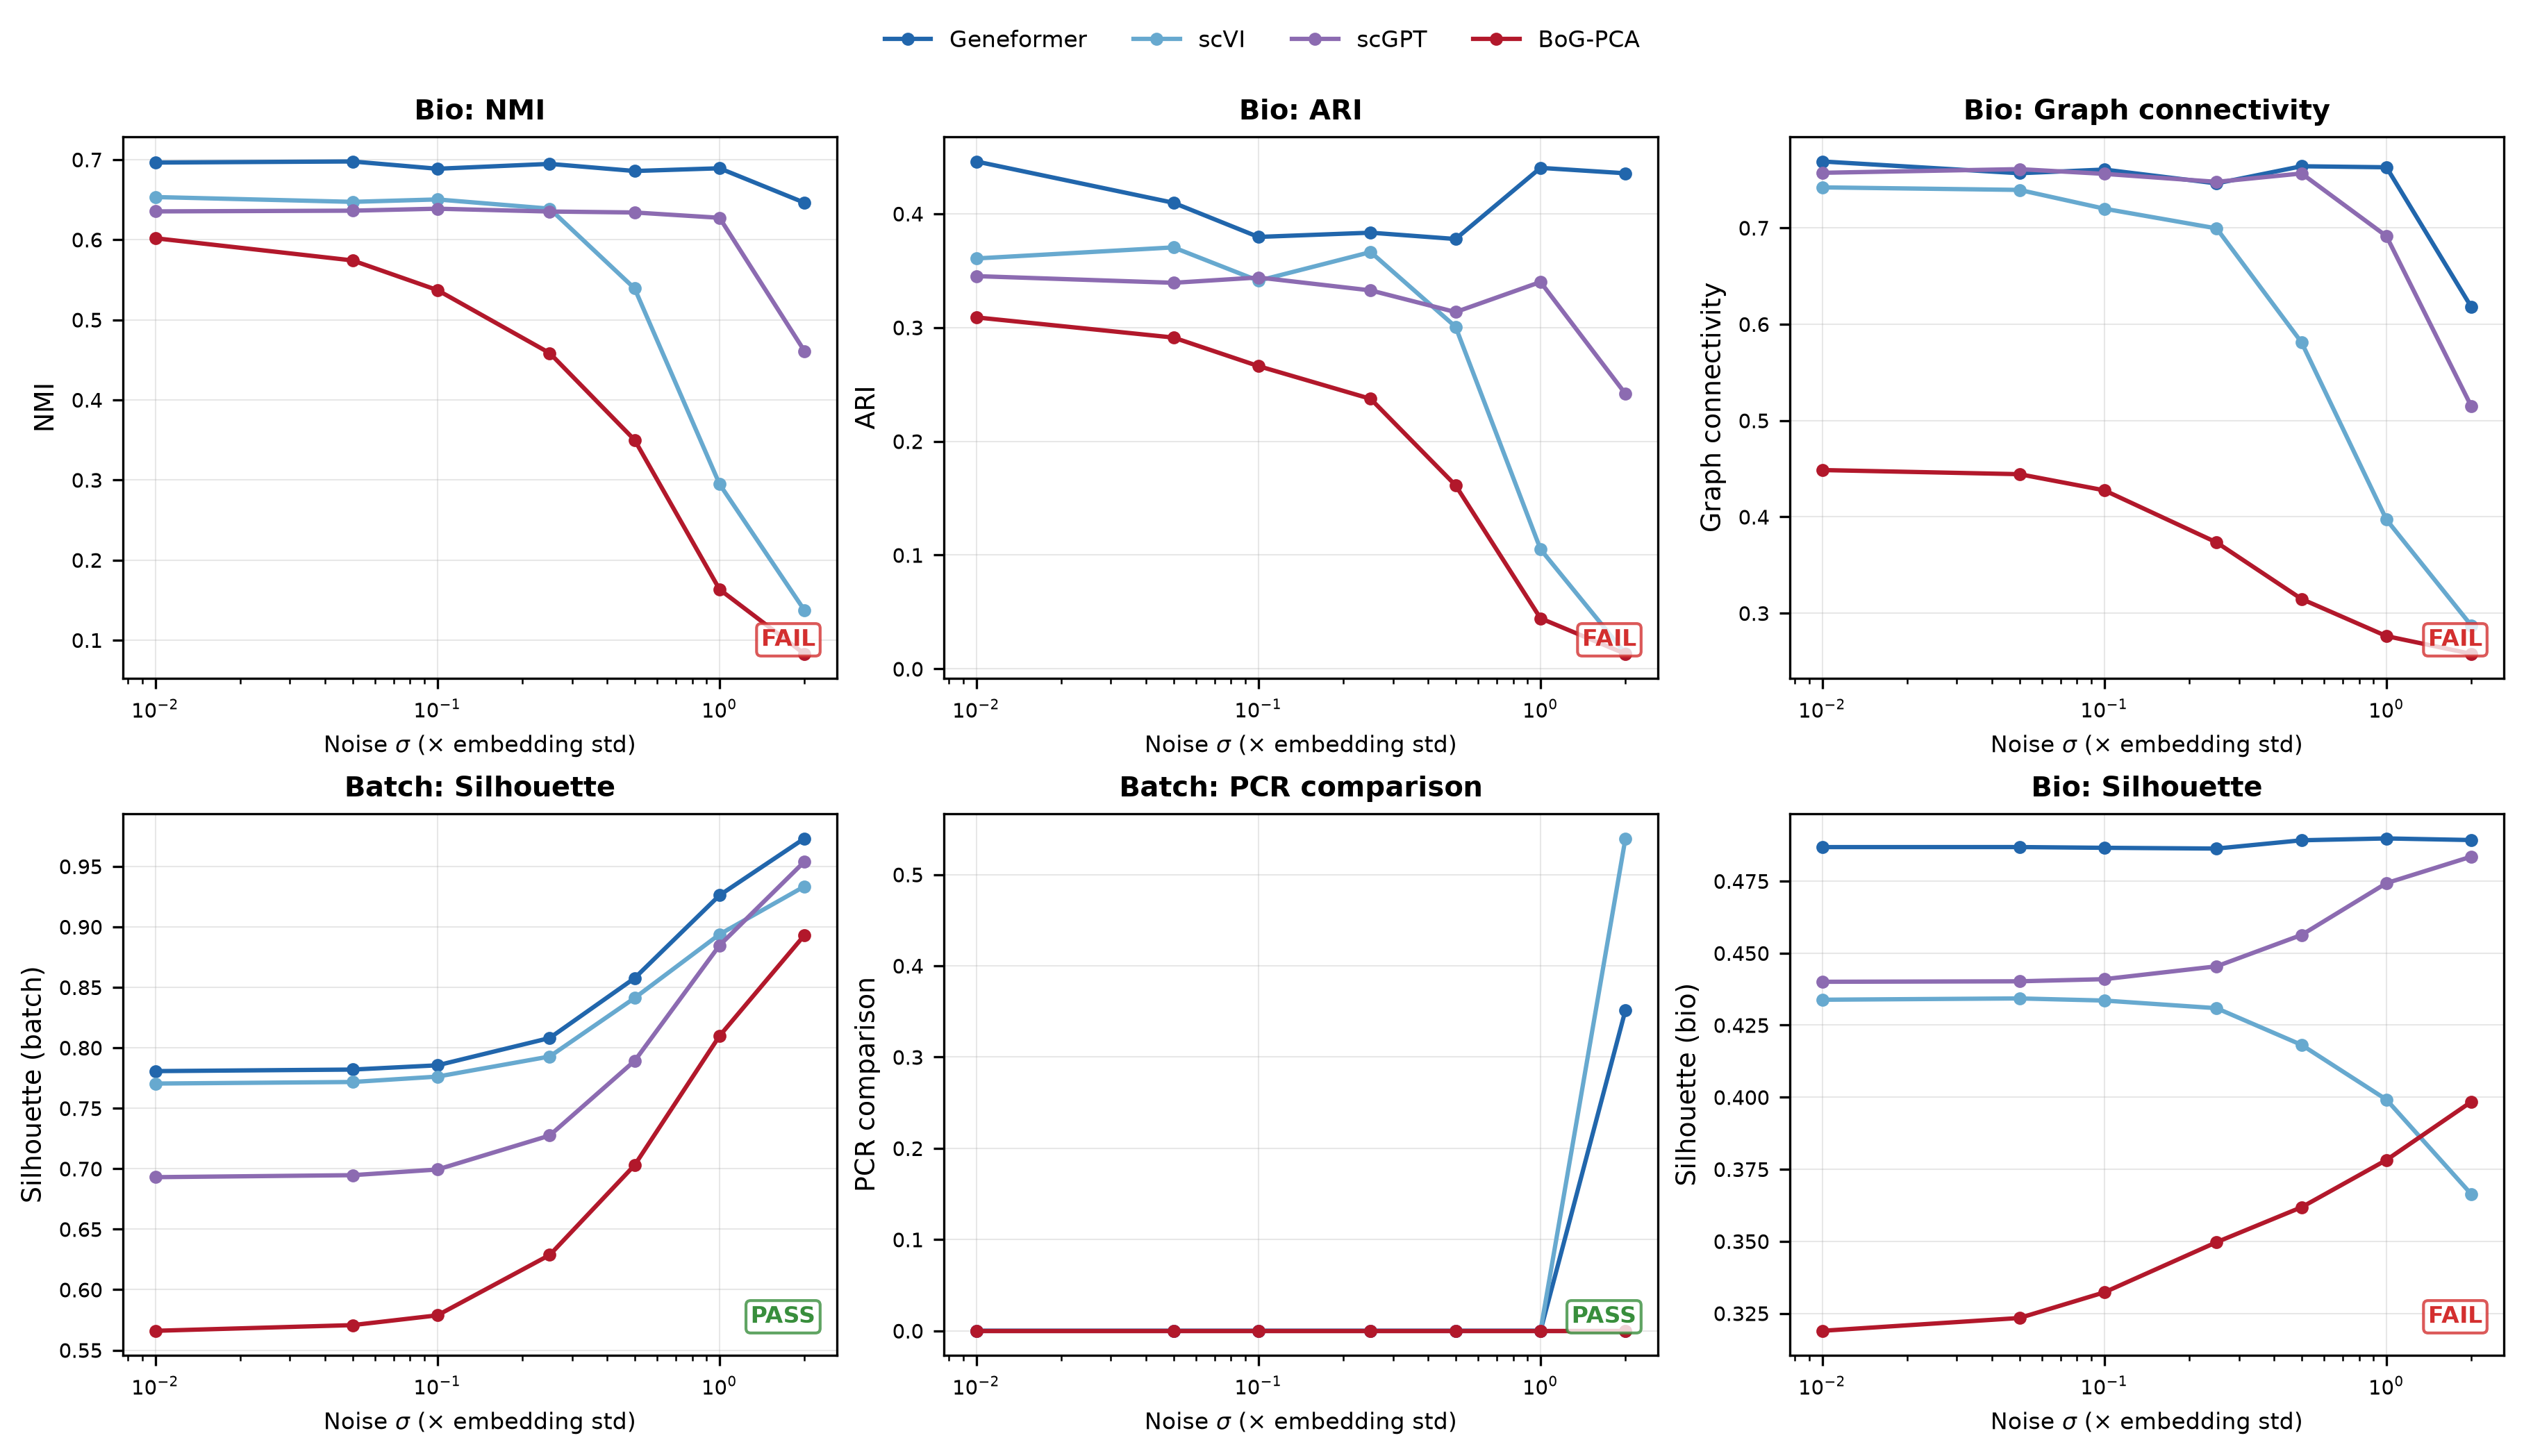
\includegraphics[width=\textwidth]{figures/noise_dose_response.pdf}
\caption{Noise dose-response curves for six scIB metrics on lung
embeddings (4 trained models). Bio-conservation metrics (top row)
show non-monotonic behavior: scores increase at intermediate noise
levels before declining, indicating sensitivity to clustering
artifacts. Batch-correction metrics (bottom center, right) decrease
monotonically as expected. Each curve traces a single embedding model
across seven noise magnitudes ($\sigma$ in units of embedding standard
deviation).}
\label{fig:noise_dose}
\end{figure}

\medskip
\begin{table}[h!]
\centering
\caption{Noise dose-response: raw vs.\ null-calibrated
non-monotonicity across 120 conditions (22 tissues $\times$ $\sim$6
embeddings, 10 seeds). Raw: fraction with mean $H > 0.01$ (metric
increased at some noise level). Calibrated: fraction exceeding the
permutation null ($\alpha = 0.01$, 1{,}000 $\sigma$-label
permutations). The inflation ratio quantifies how much uncalibrated
analysis overstates genuine non-monotonicity.}
\label{tab:noise}
\small
\begin{tabular}{@{}lccc@{}}
\toprule
Metric & Raw positive & Calibrated & Inflation \\
\midrule
ARI (Leiden)         & 84/120 (70\%) &  8/120 (6.7\%)  & 10.5$\times$ \\
Graph connectivity   & 58/120 (48\%) &  3/120 (2.5\%)  & 19.3$\times$ \\
NMI (Leiden)         & 28/120 (23\%) &  4/120 (3.3\%)  &  7.0$\times$ \\
\midrule
Cell-type CKA        & 58/120 (48\%) & 34/120 (28\%)   &  1.7$\times$ \\
Procrustes           & 56/120 (47\%) & 37/120 (31\%)   &  1.5$\times$ \\
\midrule
Isolated label ASW   & 32/120 (27\%) & 31/120 (26\%)   &  1.0$\times$ \\
Silhouette (label)   & 52/120 (43\%) & 49/120 (41\%)   &  1.1$\times$ \\
\bottomrule
\end{tabular}
\end{table}

Multi-seed calibration shows that apparent non-monotonicity in
Leiden-dependent metrics is almost entirely clustering jitter. ARI
drops from 70\% raw non-monotonic to 6.7\% after calibration
(10.5$\times$ inflation); graph connectivity drops from 48\% to 2.5\%
(19.3$\times$). Noise drives cells into fewer Leiden clusters,
mechanically raising NMI, and smooths local neighborhoods, transiently
increasing graph connectivity. These per-seed increases are real but
do not exceed what random permutation of $\sigma$ labels produces.

Similarity metrics (CKA, Procrustes) and label-based metrics
(isolated-label ASW, silhouette) show modest inflation
(1.0--1.7$\times$), indicating that their non-monotonicity, where it
occurs, reflects a genuine response to noise.

\begin{figure}[h!]
\centering
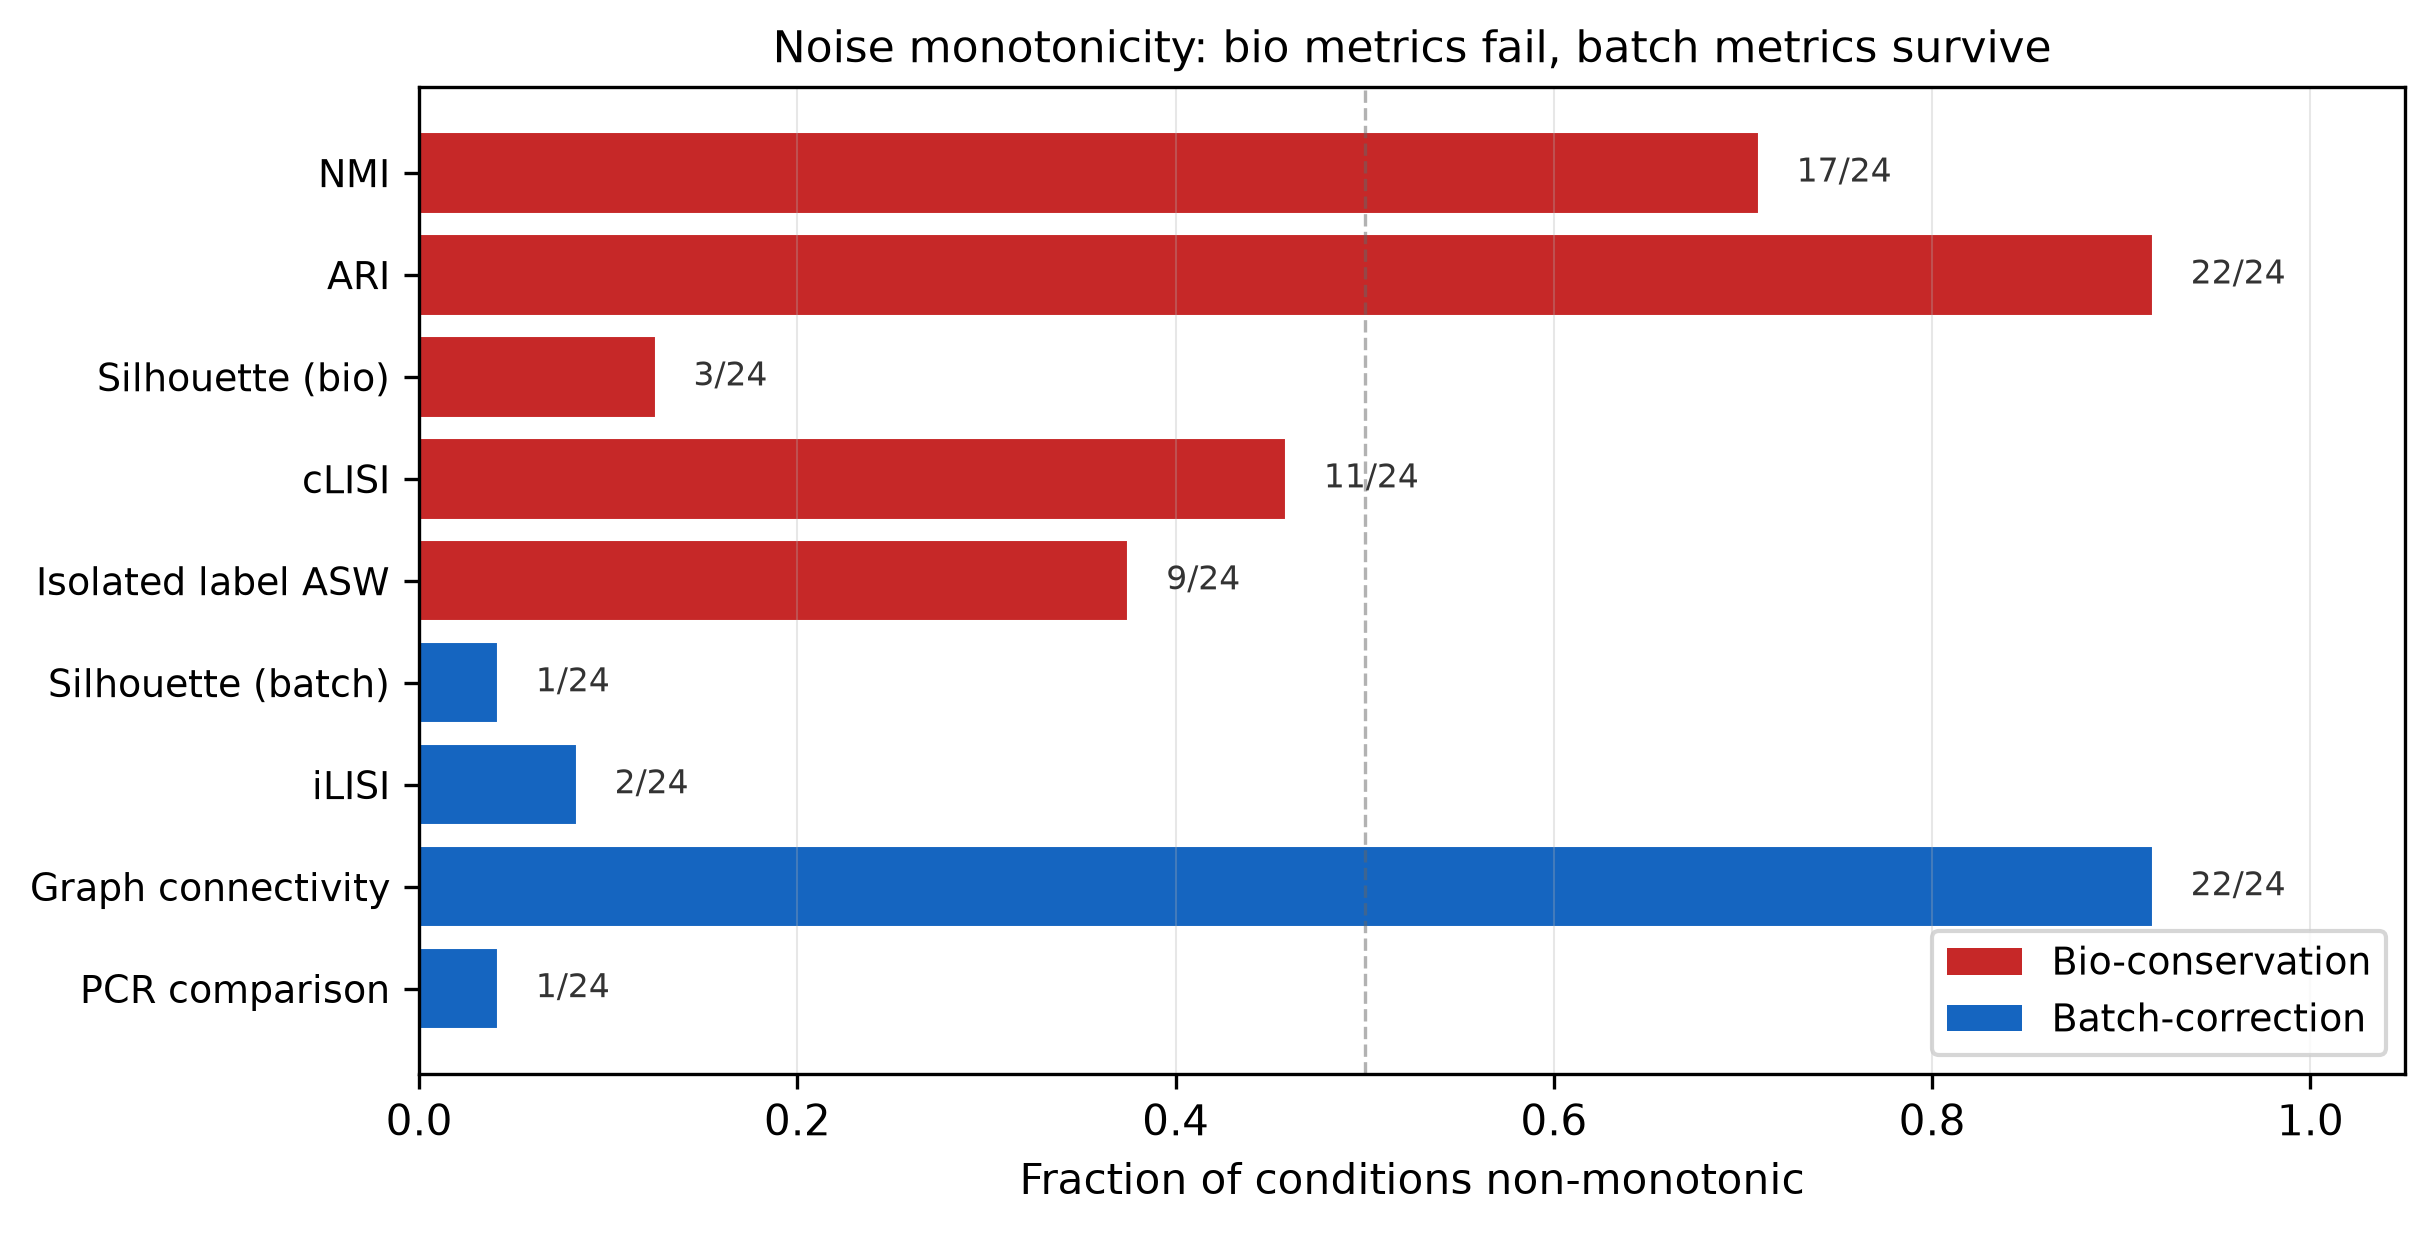
\includegraphics[width=0.85\textwidth]{figures/monotonicity_summary.pdf}
\caption{Fraction of embedding conditions (tissue $\times$ model)
exhibiting non-monotonic noise response, by metric. Bio-conservation
metrics (red) are non-monotonic in 25--75\% of conditions;
batch-correction metrics (blue) are non-monotonic in fewer than 15\%.
Counts are uncalibrated; Table~\ref{tab:noise} reports the calibrated
fractions after permutation testing.}
\label{fig:monotonicity}
\end{figure}

\paragraph{Single-seed trajectories.}
Table~\ref{tab:app_noise_fail} shows representative single-seed
non-monotonic trajectories illustrating the clustering jitter that
multi-seed calibration eliminates. NMI in brain/Geneformer shows scores
\emph{increasing} at high noise ($\sigma \geq 1.0$): noise drives all
cells into fewer Leiden clusters, mechanically raising NMI. These
per-seed trajectory changes are real but do not exceed what random
permutation of noise labels produces.

\medskip
\begin{table}[h!]
\centering
\caption{Representative single-seed non-monotonic trajectories. Values
are metric scores at $\sigma \in \{0.01, 0.05, 0.1, 0.25, 0.5, 1.0,
2.0\} \times \text{embedding\_std}$. Multi-seed calibration
(Table~\ref{tab:noise}) shows these patterns do not survive permutation
testing.}
\label{tab:app_noise_fail}
\footnotesize
\begin{tabular}{@{}llp{0.6\textwidth}@{}}
\toprule
Metric & Condition & $\sigma$: 0.01, 0.05, 0.1, 0.25, 0.5, 1.0, 2.0 \\
\midrule
Graph conn. & brain / scgpt & 0.772, 0.771, 0.773, \textbf{0.777}, \textbf{0.793}, 0.748, 0.589 \\
NMI & brain / geneformer & 0.550, 0.550, 0.545, \textbf{0.547}, 0.545, \textbf{0.575}, \textbf{0.577} \\
ARI & kidney / scvi & 0.397, \textbf{0.410}, 0.394, 0.351, 0.224, 0.073, 0.012 \\
cLISI & lung / scvi & 0.999, 0.999, \textbf{0.999}, 0.998, 0.975, 0.871, 0.642 \\
\bottomrule
\end{tabular}
\end{table}


\bibliographystyle{plainnat}
\bibliography{paper_d_v11}

\end{document}
